\documentclass[10pt]{article}

% Manage page layout
\usepackage[margin=2.5cm, includefoot, footskip=30pt]{geometry}
\pagestyle{plain}
\setlength{\parindent}{0em}
\setlength{\parskip}{1em}
\renewcommand{\baselinestretch}{1}

%%%%%%%PACKAGES HERE%%%%%%%
\usepackage{tikz}
\usepackage{amsmath}
\usepackage{amssymb}
\usepackage{amsthm}
\usepackage{graphicx}
\usepackage{subcaption}
\usepackage{standalone}
\usepackage{booktabs}
\usepackage{setspace}
\usepackage[]{algorithm2e}
\usepackage[noend]{algpseudocode}
\usepackage{wrapfig}

\makeatletter
\def\BState{\State\hskip-\ALG@thistlm}
\makeatother

\newcommand{\R}{\mathbb{R}}
\newtheorem{theorem}{Theorem}
\usetikzlibrary{decorations.pathmorphing, decorations.pathreplacing, angles,
                quotes, calc, er, positioning}

\newtheorem{lemma}[theorem]{Lemma}
\def\arraystretch{1.5}

\title{Stability of defection, optimisation of strategies and the limits of
       memory in the Prisoner's Dilemma.}
\author{Nikoleta E. Glynatsi \and Vincent A. Knight}
\date{}

\begin{document}

\maketitle

\begin{abstract}
    Memory one strategies are a set of iterated prisoner’s dilemma strategies
    that have been praised for their mathematical tractability and robustness.
    This manuscript explores \textit{best response} memory one strategies and
    studies them as a multidimensional optimisation problem. Though extortionate
    memory one strategies have gained much attention, we prove that best response
    memory one strategies do not behave in an extortionate way. For memory
    one strategies to be evolutionary robust they need to be able to behave in a
    forgiving way. We also provide evidence that memory one strategies suffer
    from the limitation of their memory and can be out performed in multi agent
    interactions by longer memory strategies.
\end{abstract}

\section{Introduction}\label{section:introduction}

The Prisoner's Dilemma (PD) is a two player game used in understanding the
evolution of co-operative behaviour, formally introduced in~\cite{Flood1958}.
Each player has two options, to cooperate (C) or to defect (D). The decisions
are made simultaneously and independently. The normal form representation of the
game is given by:

\begin{equation}\label{equ:pd_definition}
    S_p =
    \begin{pmatrix}
        R & S  \\
        T & P
    \end{pmatrix}
    \quad
    S_q =
    \begin{pmatrix}
        R & T  \\
        S & P
    \end{pmatrix}
\end{equation}

where \(S_p\) represents the utilities of the row player and \(S_q\) the
utilities of the column player. The payoffs, \((R, P, S, T)\), are constrained
by equations~(\ref{eq:pd_constrain_one}) and~(\ref{eq:pd_constrain_two}).
Constraint~(\ref{eq:pd_constrain_one}) ensures that
defection dominates cooperation and constraint~(\ref{eq:pd_constrain_two})
ensures that there is a dilemma; the sum of the utilities for both players is
better when both choose to cooperate. The most common values used in the literature are
\((3, 1, 0, 5)\)~\cite{Axelrod1981}.


\begin{equation}\label{eq:pd_constrain_one}
    T > R > P > S
\end{equation}

\begin{equation}\label{eq:pd_constrain_two}
    2R > T + S
\end{equation}

The PD is a one shot game, however it is commonly studied in a manner where the
history of the interactions matters. The repeated form of the game is called the
Iterated Prisoner's Dilemma (IPD) and in the 1980s, following the work
of~\cite{Axelrod1980a, Axelrod1980b} it attracted the attention of the
scientific community. In~\cite{Axelrod1980a} and~\cite{Axelrod1980b}, the first
well known computer tournaments of the IPD were performed. A total of 13 and 63
strategies were submitted respectively in the form of computer code. The
contestants competed against each other, a copy of themselves and a random
strategy. The winner was then decided on the average score a strategy achieved (not
the total number of wins). The contestants were given access to the entire
history of a match, however, how many turns of history a strategy would
incorporate, refereed to as the \textit{memory size} of a strategy, was a result
of the particular strategic decisions made by the author.

The winning strategy of both tournaments was the strategy called Tit for Tat.
Tit for Tat starts by cooperating and then mimics the last move of it's
opponent, more specifically, it is a strategy that considers only the previous
move of the opponent. These type of strategies are called
\textit{reactive}~\cite{Nowak1989} and are a subset of so called \textit{memory
one} strategies. Memory one strategies similarly only consider the previous
turn, however, they incorporate both players' recent moves.

Several successful reactive and memory one strategies are found in the
literature, such as Generous Tit For Tat~\cite{Nowak1990} and
Pavlov~\cite{Nowak1993}. However, memory one strategies generated a small shock
in the game theoretic community (\cite{Stewart2012} stated that ``Press and
Dyson have fundamentally changed the viewpoint on the Prisoner's Dilemma'') when
a curtain set of memory one strategies was introduced in~\cite{Press2012}. These
strategies are called zero determinate (ZD) and they chose their actions so that
a linear relationship is forced between their score and that of the opponent. ZD
strategies are indeed mathematically unique and are proven to be robust in pairwise
interactions. Their true effectiveness in tournament interactions and evolutionary
dynamics has been questioned by several works.

The purpose of this work is to consider a given memory one strategy in a similar
fashion to~\cite{Press2012}, however whilst~\cite{Press2012} found a way for a
player to manipulate a given opponent, this work will consider a
multidimensional optimisation approach to identify the best response memory one
to a group of opponents. The main questions we raise are concerned with:

\begin{itemize}
    \item A compact method of identifying the best response memory one strategy
    against a given set of opponents.
    \item The behaviour of a best response memory one strategy and whether it
    behaves extortionate, similar to ~\cite{Press2012}.
    \item The factors that make a best response memory one strategy evolutionary
    robust.
    \item A well designed framework that allows the comparison of an optimal memory
          one strategy, and a more complex strategy that has a larger memory and
          was obtained through contemporary reinforcement learning techniques.
    \item An identification of conditions for which defection is known to be
    a best response; thus identifying environments where cooperation can
    not occur.
\end{itemize}

\section{The utility}\label{section:utility}

One specific advantage of memory one strategies is their mathematical
tractability. They can be represented completely as a vector of \(\R^{4}\). This
originates from~\cite{Nowak1989} where it is stated that if a strategy is
concerned with only the outcome of a single turn then there are four possible
`states' the strategy could be in; \(CC, CD, DC,CC\). Therefore, a memory one
strategy can be denoted by the probability vector of cooperating after each of
these states; \(p=(p_1, p_2, p_3, p_4) \in \R_{[0,1]} ^ 4\). In an IPD match two
memory one strategies are moving from state to state, at each turn with a given
probability. This exact behaviour can be modeled as a stochastic process, and
more specifically as a Markov chain (Figure~\ref{fig:markov_chain}). The
corresponding transition matrix \(M\) of Figure~\ref{fig:markov_chain} is given
below,

\begin{figure}
    \begin{minipage}{0.35\textwidth}
        \includestandalone[width=\textwidth]{tex/markov_chain}
        \caption{markov}
        \label{fig:markov_chain}
    \end{minipage}
    \begin{minipage}{0.45\textwidth}
    \begin{equation*}
        M = \left[\begin{matrix}p_{1} q_{1} & p_{1} \left(- q_{1} + 1\right) & q_{1} \left(- p_{1} + 1\right) & \left(- p_{1} + 1\right) \left(- q_{1} + 1\right)\\p_{2} q_{3} & p_{2} \left(- q_{3} + 1\right) & q_{3} \left(- p_{2} + 1\right) & \left(- p_{2} + 1\right) \left(- q_{3} + 1\right)\\p_{3} q_{2} & p_{3} \left(- q_{2} + 1\right) & q_{2} \left(- p_{3} + 1\right) & \left(- p_{3} + 1\right) \left(- q_{2} + 1\right)\\p_{4} q_{4} & p_{4} \left(- q_{4} + 1\right) & q_{4} \left(- p_{4} + 1\right) & \left(- p_{4} + 1\right) \left(- q_{4} + 1\right)\end{matrix}\right]
    \end{equation*}
    \end{minipage}
\end{figure}

The long run steady state probability \(v\) is the solution to \(v M = v\). The
stationary vector \(v\) can be combined with the payoff matrices of
equation~(\ref{equ:pd_definition}) and the expected payoffs for each player
can be estimated without simulating the actual interactions. More
specifically, the utility for a memory one strategy \(p\) against an opponent \(q\),
denoted as \(u_q(p)\), is defined by,

\begin{equation}\label{eq:press_dyson_utility}
    u_q(p) = v \times (R, P, S, T).
\end{equation}

In Theorem~\ref{theorem:quadratic_form_u}, the first theoretical results of
the manuscript is presented, that is that \(u_q(p)\) is given by a ratio of
two quadratic forms~\cite{kepner2011}. To the authors knowledge this is the
first work that has been done on the form of \(u_q(p)\).

\begin{theorem}\label{theorem:quadratic_form_u}
    The expected utility of a memory one strategy \(p\in\mathbb{R}_{[0,1]}^4\)
    against a memory one opponent \(q\in\mathbb{R}_{[0,1]}^4\), denoted
    as \(u_q(p)\), can be written as a ratio of two quadratic forms:

    \begin{equation}\label{eq:optimisation_quadratic}
    u_q(p) = \frac{\frac{1}{2}pQp^T + cp + a}
                {\frac{1}{2}p\bar{Q}p^T + \bar{c}p + \bar{a}},
    \end{equation}
    where \(Q, \bar{Q}\) \(\in \R^{4\times4}\) are hollow matrices defined by the
    transition probabilities of the opponent \(q_1, q_2, q_3, q_4\) as follows:

    \begin{center}
    \begin{equation}
    \resizebox{0.9\linewidth}{!}{\arraycolsep=2.5pt%
    \boldmath\(
    Q = \left[\begin{matrix}0 & 5 q_{4} \left(q_{1} - q_{3}\right) & - q_{4} \left(q_{1} - q_{2}\right) & \left(q_{1} - q_{4}\right) \left(q_{2} - 5 q_{3} - 1\right)\\5 q_{4} \left(q_{1} - q_{3}\right) & 0 & - 3 q_{4} \left(q_{2} - q_{3}\right) & \left(q_{3} - q_{4}\right) \left(5 q_{1} - 3 q_{2} - 2\right)\\- q_{4} \left(q_{1} - q_{2}\right) & - 3 q_{4} \left(q_{2} - q_{3}\right) & 0 & - \left(q_{2} - q_{4}\right) \left(q_{1} - 3 q_{3} - 1\right)\\\left(q_{1} - q_{4}\right) \left(q_{2} - 5 q_{3} - 1\right) & \left(q_{3} - q_{4}\right) \left(5 q_{1} - 3 q_{2} - 2\right) & - \left(q_{2} - q_{4}\right) \left(q_{1} - 3 q_{3} - 1\right) & 0\end{matrix}\right]\)},
    \end{equation}
    \begin{equation}\label{eq:q_bar_matrix}
    \resizebox{0.8\linewidth}{!}{\arraycolsep=2.5pt%
    \boldmath\(
    \bar{Q} =  \left[\begin{matrix}0 & - \left(q_{1} - q_{3}\right) \left(q_{2} - q_{4} - 1\right) & \left(q_{1} - q_{2}\right) \left(q_{3} - q_{4}\right) & \left(q_{1} - q_{4}\right) \left(q_{2} - q_{3} - 1\right)\\- \left(q_{1} - q_{3}\right) \left(q_{2} - q_{4} - 1\right) & 0 & \left(q_{2} - q_{3}\right) \left(q_{1} - q_{4} - 1\right) & \left(q_{1} - q_{2}\right) \left(q_{3} - q_{4}\right)\\\left(q_{1} - q_{2}\right) \left(q_{3} - q_{4}\right) & \left(q_{2} - q_{3}\right) \left(q_{1} - q_{4} - 1\right) & 0 & - \left(q_{2} - q_{4}\right) \left(q_{1} - q_{3} - 1\right)\\\left(q_{1} - q_{4}\right) \left(q_{2} - q_{3} - 1\right) & \left(q_{1} - q_{2}\right) \left(q_{3} - q_{4}\right) & - \left(q_{2} - q_{4}\right) \left(q_{1} - q_{3} - 1\right) & 0\end{matrix}\right]\)}.
    \end{equation}
    \end{center}

    \(c \text{ and } \bar{c}\) \(\in \R^{4 \times 1}\) are similarly defined by:

    \begin{equation}\label{eq:q_matrix_numerator}
    \resizebox{0.3\linewidth}{!}{\arraycolsep=2.5pt%
    \boldmath\(c = \left[\begin{matrix}- 5 q_{1} q_{4}\\5 q_{4} \left(q_{3} - 1\right)\\q_{4} \left(2 q_{2} + 1\right)\\5 q_{1} q_{4} - 2 q_{2} q_{4} - q_{2} - 5 q_{3} q_{4} + 5 q_{3} - 3 q_{4} + 1\end{matrix}\right]\),}
    \end{equation}
    \begin{equation}\label{eq:q_matrix_denominator}
    \resizebox{0.3\linewidth}{!}{\arraycolsep=2.5pt%
    \boldmath\(\bar{c} = \left[\begin{matrix}q_{1} \left(q_{2} - q_{4} - 1\right)\\- \left(q_{3} - 1\right) \left(q_{2} - q_{4} - 1\right)\\- q_{1} q_{2} + q_{2} q_{3} + q_{2} - q_{3} + q_{4}\\q_{1} q_{4} - q_{2} - q_{3} q_{4} + q_{3} - q_{4} + 1\end{matrix}\right]\).
    }
    \end{equation}
    and \(a = 5 q_{4}\) and
    \(\bar{a} = - q_{2} + q_{4} + 1\).
\end{theorem}

The proof of Theorem~\ref{theorem:quadratic_form_u} is given in Appendix. %TODO write proof

Numerical simulations have been carried out to validate the formulation of
\(u_q(p)\) as a quadratic ratio, a data set is available at.
Figure~\ref{fig:analytical_simulated} shows that the formulation successfully
captures the simulated behaviour. The simulated utility, which is denoted as
\(U_q(p)\), has been calculated using~\cite{axelrodproject} an open source
research framework for the study of the IPD. The project is described
in~\cite{Knight2016}. All of the aforementioned simulated results have been
estimated using~\cite{axelrodproject}.

\begin{figure}[!htbp]
    \begin{center}
        \begin{subfigure}{0.45\textwidth}
            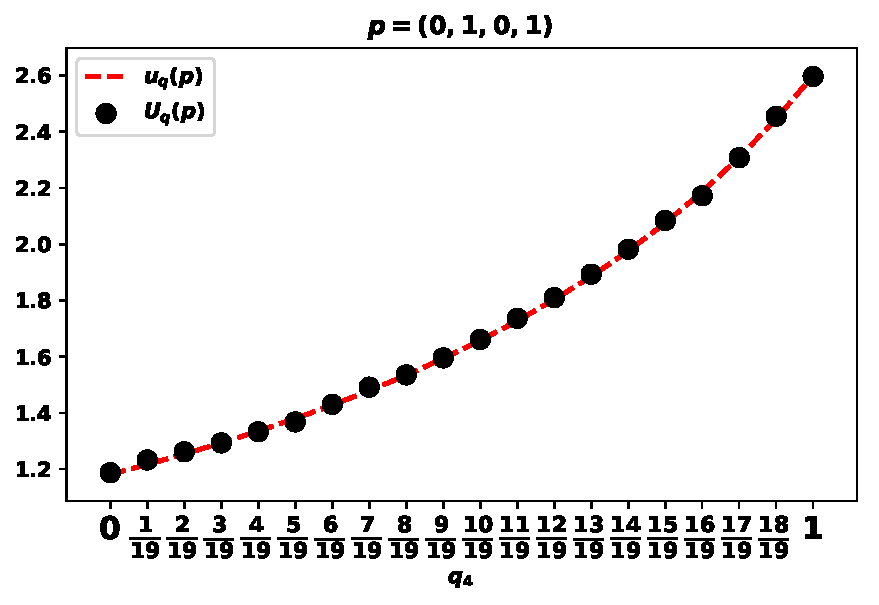
\includegraphics[width=\linewidth]{img/validation_against_player_one.pdf}
        \end{subfigure}
        \begin{subfigure}{0.45\textwidth}
            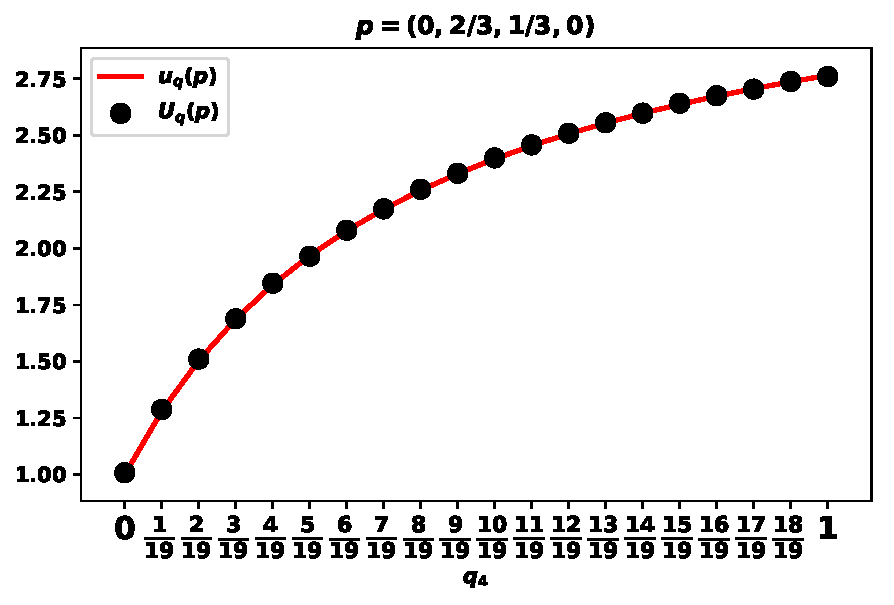
\includegraphics[width=\linewidth]{img/validation_against_player_two.pdf}
        \end{subfigure}
    \end{center}

    \caption{Differences between simulated and analytical results for
            \(q = (\frac{1}{3}, \frac{1}{3}, \frac{1}{3}, q_4)\).}
    \label{fig:analytical_simulated}
\end{figure}

Theorem~\ref{theorem:quadratic_form_u} can be extended to consider multiple
opponents. The IPD is commonly studied in tournaments and/or Moran Processes
where a strategy interacts with a number of opponents. The payoff of a player in
such interactions is given by the average payoff the player received against
each opponent. More specifically the expected utility of a memory one strategy
against a \(N\) number of opponents is given by
Theorem~\ref{theorem:tournament_utility}.

\begin{theorem}\label{theorem:tournament_utility}
    The expected utility of a memory one strategy \(p\in\mathbb{R}_{[0,1]}^4\)
    against a group of opponents \(q^{(1)}, q^{(2)}, \dots, q^{(N)}\), denoted
    as \(\frac{1}{N} \sum\limits_{i=1} ^ {N} {u_q}^{(i)} (p)\) is given by:

    \begin{equation}\label{eq:tournament_utility}
        \frac{1}{N} \sum\limits_{i=1} ^ {N} {u_q}^{(i)} (p) = \frac{1}{N}
        \frac{\sum\limits_{i=1} ^ {N} (\frac{1}{2} pQ^{(i)} p^T + c^{(i)} p + a^ {(i)})
        \prod\limits_{\tiny\begin{array}{l} j=1 \\ j \neq i \end{array}} ^
        N (\frac{1}{2} p\bar{Q}^{(i)} p^T + \bar{c}^{(i)} p + \bar{a}^ {(i)})}
        {\prod\limits_{i=1} ^ N (\frac{1}{2} p\bar{Q}^{(i)} p^T + \bar{c}^{(i)} p + \bar{a}^ {(i)})}.
    \end{equation}
\end{theorem}

Theorem~\ref{theorem:tournament_utility} is validated against the strategies
used in~\cite{Stewart2012}, Figure~\ref{fig:stewart_plotkin_results}. The
list of strategies from~\cite{Stewart2012} alonside their original reference from the 
are given by Table~\ref{table:list_stewart_plotkin} in the Appendix.

\begin{figure}[!htbp]
    \begin{center}
    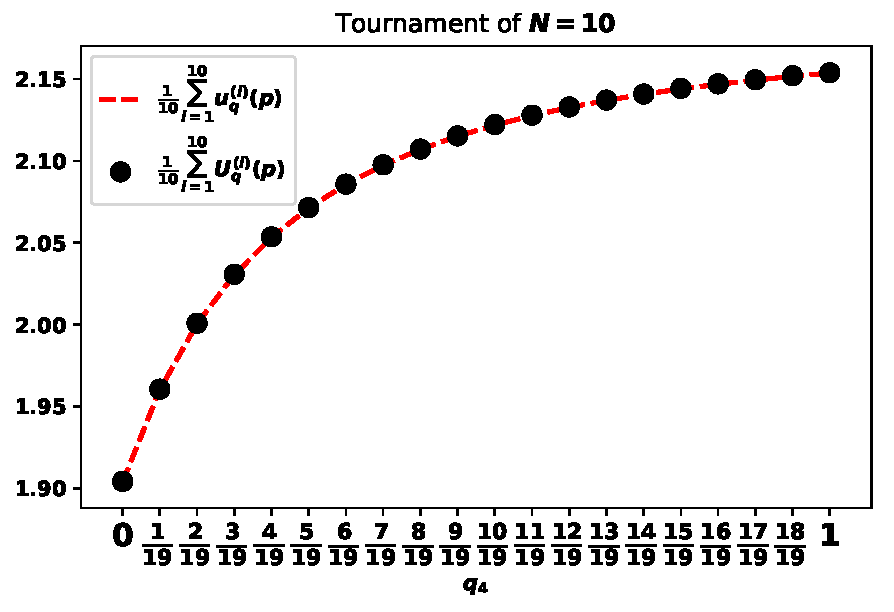
\includegraphics[width=.5\linewidth]{img/Stewart_tournament_results.pdf}
    \caption{Results of memory one strategies against the strategies in
    Table~\ref{table:list_stewart_plotkin}.}
    \label{fig:stewart_plotkin_results}
    \end{center}
\end{figure}

Furthermore, using the same list of strategies the 
hypothesis the utility against a group of strategies could be
captured by the utility against the mean opponent, thus:

\begin{equation}\label{eq:condition}
    \frac{1}{N} \sum_{i=1} ^ {N} {u_q}^{(i)} (p) = u_{\frac {1}{N} \sum\limits_{i=1} ^ N q^{(i)}}(p),
\end{equation}

has been checked. The hypothesis fails and numerical evidence are given by
Figure~\ref{fig:hypothesis}.

\begin{figure}[!htbp]
    \begin{center}
    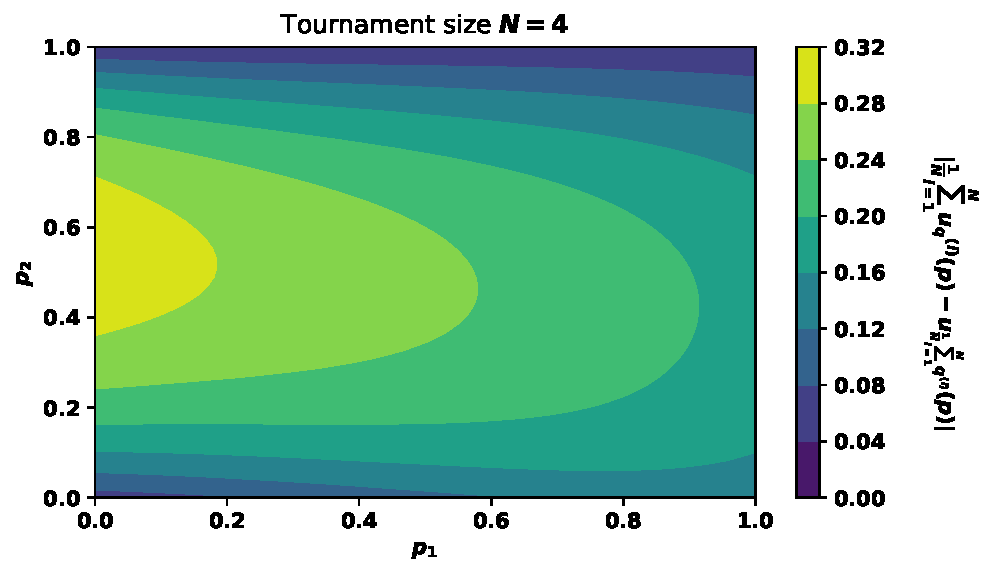
\includegraphics[width=.5\linewidth]{img/mean_vs_average_heatmap.pdf}
    \end{center}
    \caption{The difference between the average utility and against
    the utility against the average player of the strategies in~\cite{Stewart2012}.
    A positive difference indicates that the condition (\ref{eq:condition})
    does not hold.}
    \label{fig:hypothesis}
\end{figure}

Theorem~\ref{theorem:tournament_utility} can be used to identify best
responses in the case of memory one strategies. In the following sections several
theoretical results are presented and the advantages of analytical formulation
of become evident.

\section{Best responses to memory one players}\label{section:best_response_mem_one}

A \textit{best response} is the strategy which corresponds to the most
favourable outcome. A best response memory one strategy
corresponds to the \(p^*\) for which \(\sum u_{q ^{(i)}} (p^*)\) for \(i \in \{1, \dots, N\}\)
is maximized. This is considered as a multi dimensional optimisation problem
where the decision variable is the vector \(p\), the solitary constraint is
that \(p \in \R^4_{[0, 1]} \) and the objective function is a sum of quadratic
ratios. The optimisation problem is formally given by~(\ref{eq:mo_tournament_optimisation}).

\begin{equation}\label{eq:mo_tournament_optimisation}
    \begin{aligned}
    \max_p: & \ \sum_{i=1} ^ {N} {u_q}^{(i)} (p)
    \\
    \text{such that}: & \ p \in \R_{[0, 1]}
    \end{aligned}
\end{equation}

Optimising this particular ratio of quadratic forms is not trivial. It can be
verified empirically for the case of a single opponent that there exist at least
one point for which the definition of concavity does not hold. Though 
\cite{Beck2009, Hongyan2014} are also concerned with a non concave ratios of
quadratic forms, in both the numerator and the denominator of
the fractional problem were concave or that the denominator was greater than
zero; both assumptions fail here. These results are established in
Theorem~\ref{theorem:concavity}.

\begin{theorem}\label{theorem:concavity}
    The utility of a player \(p\) against an opponent \(q\), \(u_q (p)\) given by
    (\ref{eq:optimisation_quadratic}), is not concave. Furthermore neither the
    numeration or the denominator of (\ref{eq:optimisation_quadratic}), are concave.
\end{theorem}

The non concavity of \(u(p)\) indicates multiple local optimal points. The
approach taken here is to introduce a compact way of constructing the candidate
set of all local optimal points. Once the set is defined the point that
maximises (\ref{eq:tournament_utility}) corresponds to the best response
strategy, this approach transforms the continuous optimisation problem in to a
discrete problem. The problem considered is a bounded because \(p \in \R^4_{[0,
1]}\). The candidate solutions will exist either at the boundaries of the
feasible solution space, or within that space. The method of Lagrange
Multipliers~\cite{bertsekas2014} and Karush-Kuhn-Tucker
conditions~\cite{Giorgi2016} are based on this.

These lead to Lemma~\ref{lemma:memone_group_best_response} which
presents the best response memory one strategy to a group of opponents.

\begin{lemma}\label{lemma:memone_group_best_response}

    The optimal behaviour of a memory one strategy player
    \(p^* \in \R_{[0, 1]} ^ 4\)
    against a set of \(N\) opponents \(\{q^{(1)}, q^{(2)}, \dots, q^{(N)} \}\)
    for \(q^{(i)} \in \R_{[0, 1]} ^ 4\) is established by:

    \[p^* = \textnormal{argmax}(\sum\limits_{i=1} ^ N  u_q(p)), \ p \in S_q.\]

    The set \(S_q\) is defined as all the possible combinations of:

    \begin{itemize}
    \item Any one, two, three, four or non of the transition probabilities of
    \(p\) are 0,
    \item while any one, two, three, four or non of the transition probabilities of
    \(p\) are 1,
    \item while any one, two, three, four or non of the transition probabilities of
    \(p\) are the roots of \(\frac{d}{dp} \sum\limits_{i=1} ^ N  u_q(p)\).
    \end{itemize}

    The derrivate \(\frac{d}{dp} \sum\limits_{i=1} ^ N  u_q(p)\) is given by:

    {\scriptsize
    \begin{align}\label{eq:mo_tournament_derivative}
        \frac{d}{dp} \sum\limits_{i=1} ^ {N} {u_q}^{(i)} (p) & = \nonumber \\
        & =\frac{
        (\sum\limits_{i=1} ^ {N} Q_{N}^{(i)'} \prod_{\substack{j=1 \\ j \neq i}} ^ N Q_{D}^{(i)}
        + \sum\limits_{i=1} ^ {N} Q_{D}^{(i)'} \sum_{\substack{j=1 \\ j \neq i}} ^ {N} Q_{N}^{(i)}
       \prod_{\substack{j=1 \\ j \neq \{i, j\}}} ^ N Q_{D}^{(i)}) \times
       \prod\limits_{i=1} ^ N Q_{D}^{(i)} - (\sum\limits_{i=1} ^ {N} Q_{D}^{(i)'}y-vk
       \prod_{\substack{j=1 \\ j \neq i}} ^ N Q_{D}^{(i)}) \times
       (\sum\limits_{i=1} ^ {N} Q_{N}^{(i)} \prod_{\substack{j=1 \\ j \neq i}} ^ N Q_{D}^{(i)})}
        {(\prod\limits_{i=1} ^ N Q_{D}^{(i)})^{2}}
    \end{align}
    }
\end{lemma}

Proof in the Appendix.

Constructing the subset \(S_q\) is analytical possible. The points for any or
none of \(p_i \in \{0, 1\}\) for \(i \in {1, 2, 3, 4}\) are trivial. Finding the
roots of the partial derivates \(\frac{d}{dp} \sum\limits_{i=1} ^ N  u_q(p)\)
is feasible using resultant theory. Resultant theory~\cite{Jonsson2005} allow
us to solve systems of polynomials by the calculation of a resultant.
However, for large systems these quickly become intractable. Because of that no
further analytical consideration is given to problems described here.

So far we have provided an analytical formulation that can estimate best response
memory one strategies against a number of opponents. This
will be revisited and solved numerically in Section~\cite{section:numerical_experiments}.
In the following subsection we present a theoretical results which has been
possible due to the formulation discussed here.

\subsection{Stability of defection}

Defection is known to be the dominant action in the PD and it can be proven to
be the dominant strategy for the IPD for given environments. Even so, several
works have proven that cooperation emerges in the IPD and many studies focus on
the emergence of cooperation. 

An immediaty results from the our formulation of best response memory one strategies
is that we can provide an identification of
conditions for which defection is known to be a best response; thus identifying
environments where cooperation can not occur.

The results are presented in Lemma~\ref{lemma:stability_of_defection}.

\begin{lemma}\label{lemma:stability_of_defection}
    In a tournament of \(N\) players where \(q^{(i)} = (q_{1}^{(i)}, q_{2}^{(i)}, q_{3}^{(i)}, q_{4}^{(i)})\)
    defection is a best response if the transition probabilities of the
    opponents satisfy the condition:

    \begin{equation}
        \sum_{i=1} ^ N (c^{(i)T} \bar{a}^{(i)} - \bar{c}^{(i)T} a^{(i)}) \leq 0
    \end{equation}
\end{lemma}

\begin{proof}
    For defection to be evolutionary stable the derivative of the utility
    at the point \(p = (0, 0, 0, 0)\) must be negative. This would indicate that
    the utility function is only declining from that point onwards.

    Substituting \(p = (0, 0, 0, 0)\) in
    equation~(\ref{eq:mo_tournament_derivative}) which gives:

    \begin{equation}
    \sum_{i=1} ^ N (c^{(i)T} \bar{a}^{(i)} - \bar{c}^{(i)T} a^{(i)})
    \prod\limits_{\tiny\begin{array}{l} j=1 \\ j \neq i \end{array}} ^ N (\bar{a}^{(i)})^2
    \end{equation}
    
    The second term \(\prod\limits_{\tiny\begin{array}{l} j=1 \\ j \neq i
    \end{array}} ^ N (\bar{a}^{(i)})^2\) is always positive, however, the sign of the
    first term \(\sum_{i=1} ^ N (c^{(i)T} \bar{a}^{(i)} - \bar{c}^{(i)T} a^{(i)})\)
    can vary based on the transition probabilities of the opponents. Thus the
    sign of the derivative is negative if and only if
    \(\sum_{i=1} ^ N (c^{(i)T} \bar{a}^{(i)} - \bar{c}^{(i)T} a^{(i)}) \leq 0\).
\end{proof}

\section{Numerical experiments} \label{section:numerical_experiments}

In this section best responses are explored numerically. Best responses are
estimated using the Bayesian optimisation algorithm, which is a
global optimisation algorithm, introduced in~\cite{Mokus1978}, that has proven
to outperform many other popular algorithms~\cite{Jones2001}. Differential
evolution had also been considered, however it was not chosen due to Bayesian
being computationally faster.

Bayesian optimisation tries to find values for the decision variables for which
the utility of a player is maximised, over a given time of calls. Consider
the problem of (\ref{eq:mo_tournament_optimisation}) where \(N=2\) and \(p^*\)
is being estimated. Figure~\ref{bayesian_example} illustrates
the change of the utility function over number of calls.
The default number of iterations that have been used in this work is 60. After
the 60 calls the convergence of the utility is checked. If it is not then the
calls are increased by 20, this step is then repeated until utility reaches
convergence.

\begin{figure}[!htbp]
    \begin{center}
    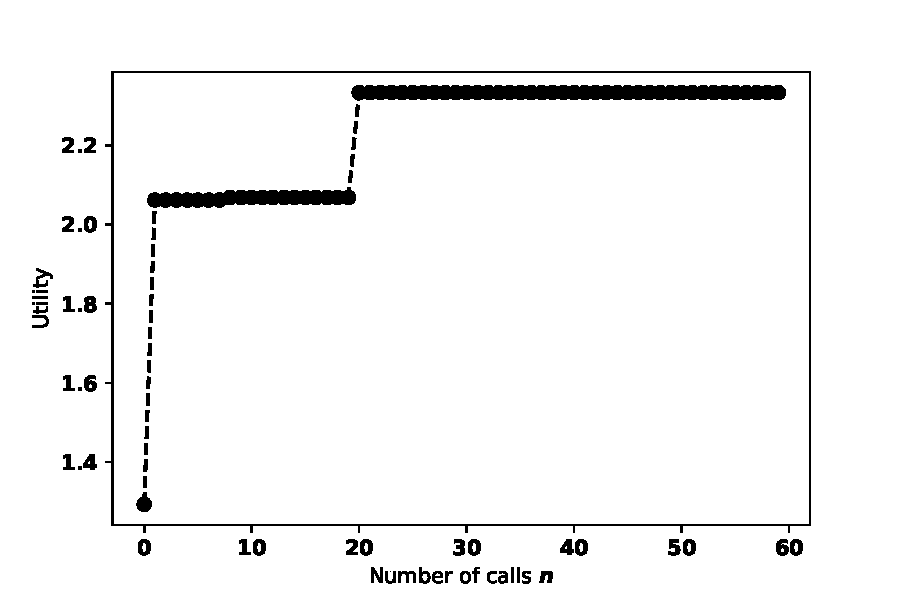
\includegraphics[width=.5\linewidth]{img/bayesian_example.pdf}
    \end{center}
    \caption{Utility over time of calls using Bayesian optimisation. The
    opponents are \(q^{(1)} = (\frac{1}{3}, \frac{1}{3}, \frac{1}{3},
    \frac{1}{3})\) and \(q^{(2)} = (\frac{1}{3}, \frac{1}{3},
    \frac{1}{3}, \frac{1}{3})\).}
    \label{bayesian_example}
\end{figure}

We will be Bayesian optimisation not only to estimate best response memory one
strategies but a series of cases are going to be explored. Evolutionary memory
one and longer memory best responses are also considered here. This is done so
we can gain a better understanding of memory one strategies, their behaviour,
robustness and limitations.

\subsection{Best response memory one strategies for \(N=2\)}\label{subsection:best_response_n_2}

The first case considered is that of best response memory one strategies in tournaments
in order to understand whether best respones behave in an extortionate way. A
large data set of best response memory one strategies when \(N=2\) has been
generated and is available here. \(N=2\) has been chosen as it's
the smallest size of a tournament.

The data set contains a total of 1000 trials and 1000 different best responses.
For each trial a set of 2 opponents is randomly generated, the memory one best
response against them is estimated and it's behaviour is being recorded.
Though the probabilities \(q_i\) of the opponents are randomly generated,
Figures~\ref{fig:first_opponents_probabilities} and \ref{fig:second_opponents_probabilities}
they are uniformly distributed over the trial. Thus, the space full space of
possible opponents has been covered.

\begin{figure}[!htbp]
    \begin{subfigure}{0.49\textwidth}
        \centering
        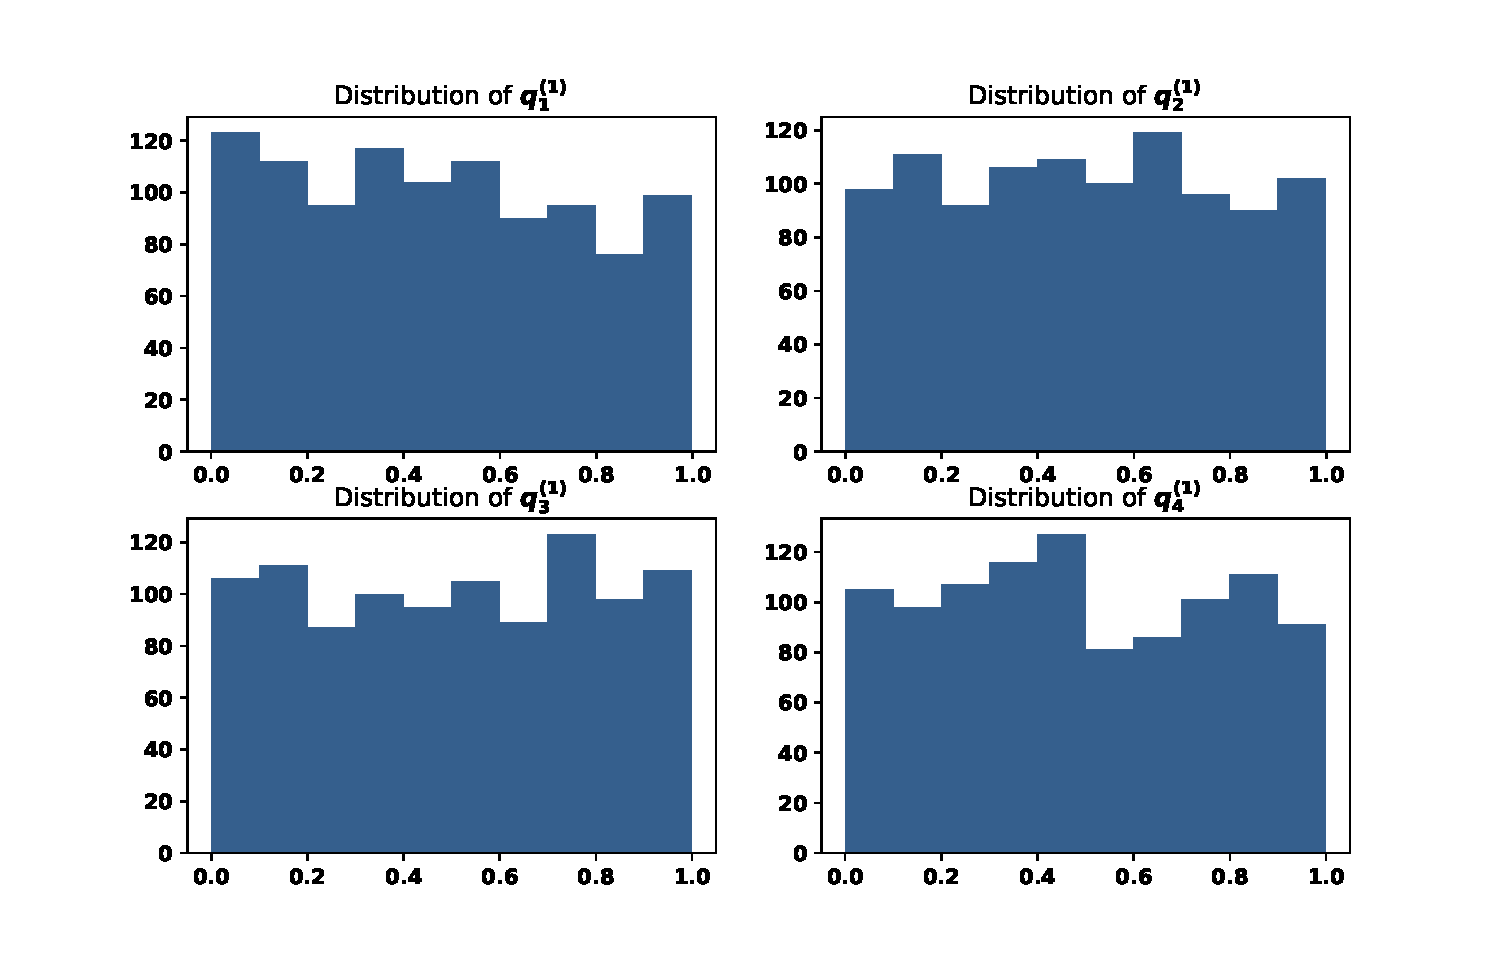
\includegraphics[width=\linewidth]{img/first_opponent_probabilities.pdf}
        \subcaption{Distributions of first opponents' probabilities.}
        \label{fig:first_opponents_probabilities}
    \end{subfigure}
    \begin{subfigure}{0.49\textwidth}
        \centering
        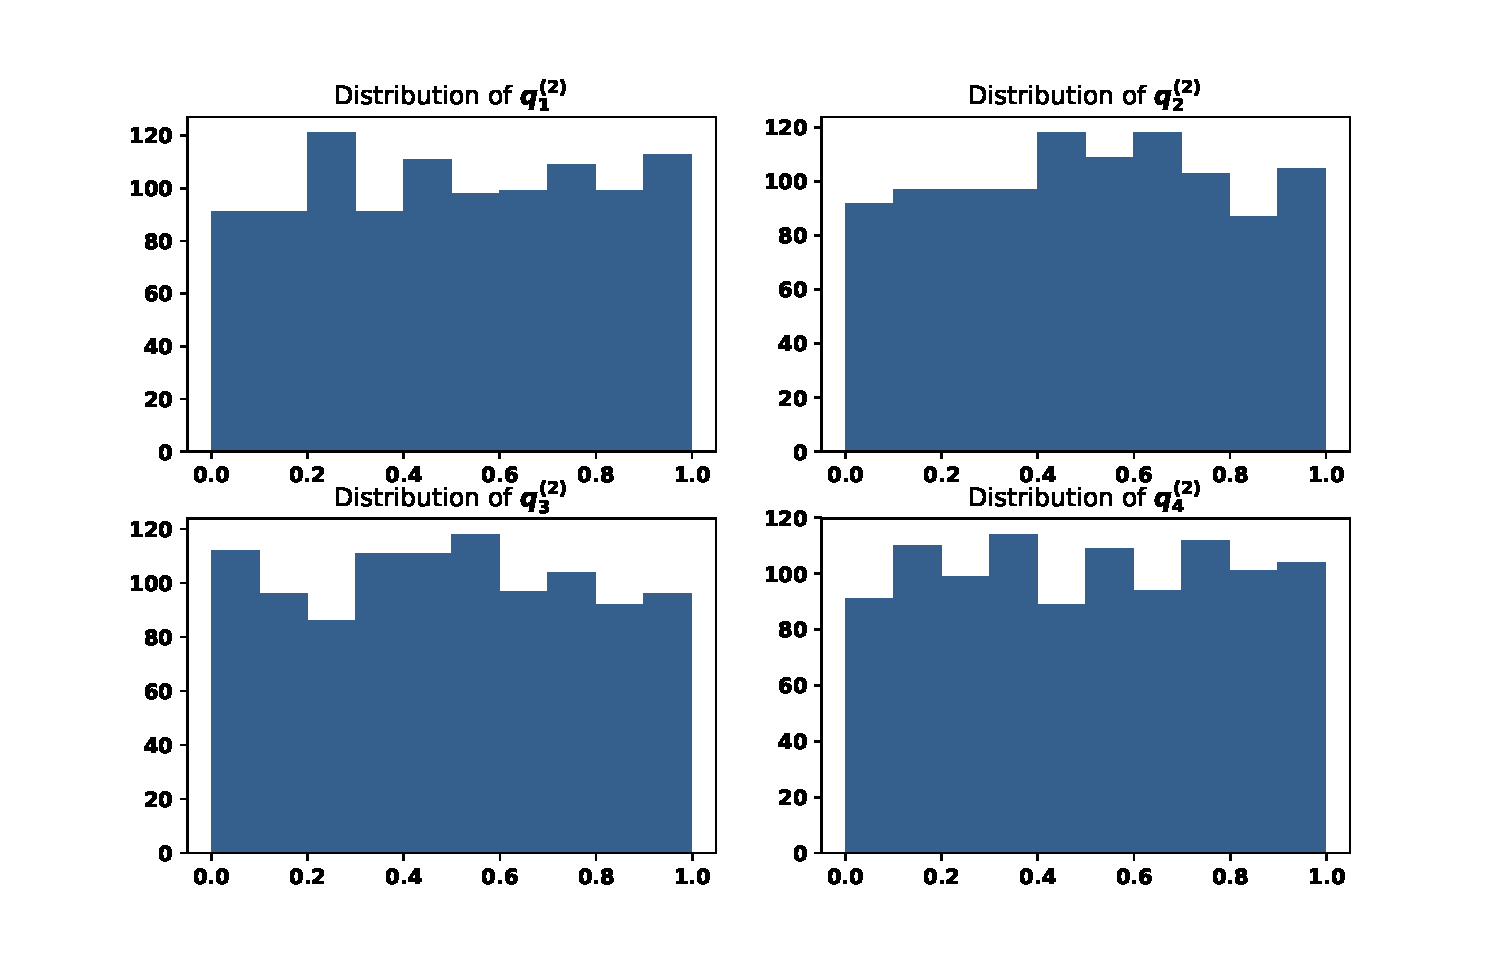
\includegraphics[width=\linewidth]{img/second_opponent_probabilities.pdf}
        \subcaption{Distributions of second opponents' probabilities.}
        \label{fig:second_opponents_probabilities}
    \end{subfigure}
\end{figure}

It was briefly discussed in Section~\ref{section:introduction} that ZD strategies
have received praised for their robustness against a single opponent. By forcing
a linear relationship between the scores ZD strategies will always manage to
receive a higher payoff than their opponents. In tournament setting the winner
is defined by the average score a strategy received, thus winning against your
opponent at each interaction does not guaranty a strategy's overall win.
This manuscript argues that by trying to exploit their opponents ZD strategies suffer in
multi opponent interaction where the payoffs matter. Compared to ZD best response
memory one strategies utilise their behaviour to gain the most from their interactions.


\begin{minipage}{0.65\linewidth}
In [Knight 2019] the authors provied a method of measuring the extortionate behaviour of a
strategy based on it's estimated probabilities. The method estimates the error of
behaving as a ZD strategy defined as SSerror. The SSerror method is applied on the
data set that has been generated in order to gain an understanding whether best
reponses memory one strategies behave in an extortionate way.
The distribution of the SSerror is shown in Figure~\ref{fig:sserror_mem_one} and
a statistics summary by Table~\ref{table:sserror_stats}. Only the 30\% of the
best responses have a SSerror less than a 0.10 and a positive measure of skewness
\((=1.96)\), indicates that the distribution is skewed to the right.
\end{minipage}
\begin{minipage}{0.39\textwidth}
    \centering
    \captionsetup{type=table}
    \resizebox{.4\columnwidth}{!}{%
        \begin{tabular}{lr}
\toprule
{} &    SSerror \\
\midrule
count  &  474.00000 \\
mean   &    0.32869 \\
std    &    0.38300 \\
min    &    0.00000 \\
5\%     &    0.02077 \\
25\%    &    0.08128 \\
50\%    &    0.16964 \\
95\%    &    1.05882 \\
max    &    2.47059 \\
median &    0.16964 \\
skew   &    1.76038 \\
kurt   &    2.70693 \\
\bottomrule
\end{tabular}
}
        \caption{Summary statistics SSerror}
        \label{table:sserror_stats}
\end{minipage}


\begin{figure}
    \begin{center}
    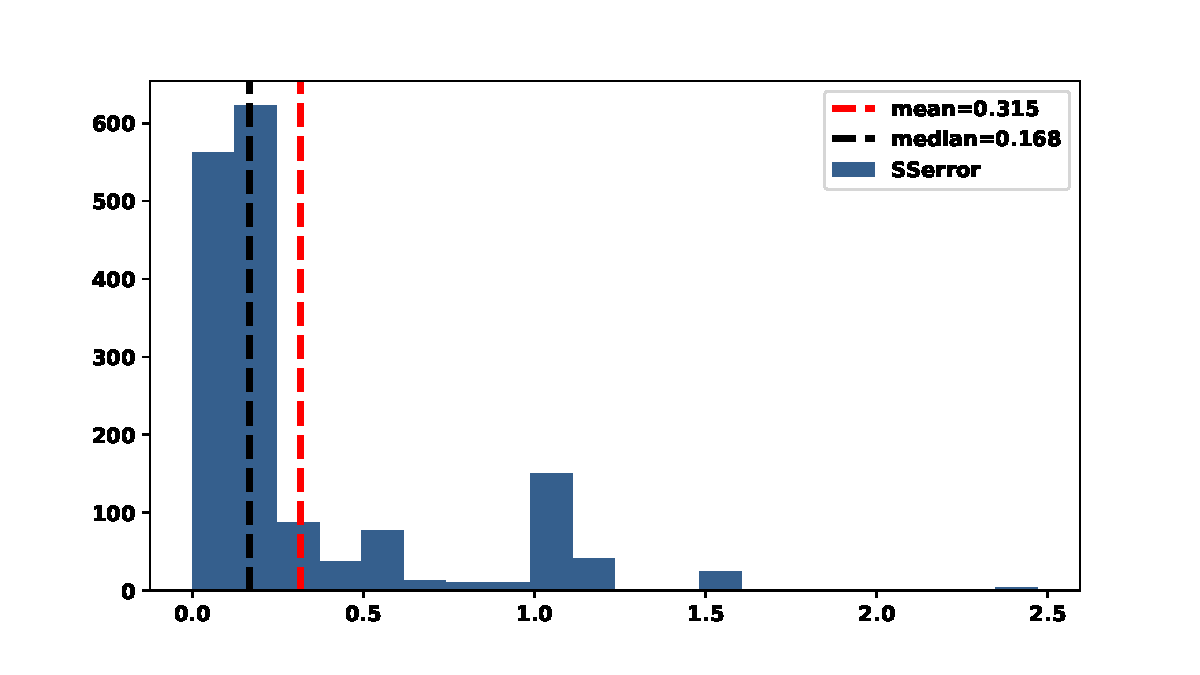
\includegraphics[width=.6\linewidth]{img/best_respones_sserror.pdf}
    \end{center}
    \caption{Distribution of sserrors for memory one best responses, when \(N=2\).}
    \label{fig:sserror_mem_one}
\end{figure}

Overall only a very small percentage of the best responses seem to behaving in
an extortionate way, confirming our original hypothesis. To gain the most of our
environment you would avoid being extortionate. The following section the second
experiment and the result of memory one best responses in evolutionary dynamics
are presented.

\newpage

\subsection{Memory one best responses in evolutionary dynamics}

As briefly discussed in Section~\ref{section:utility}, the IPD is commonly
studied in Moran Processes, and generally in evolutionary processes. In
evolutionary processes, a finite population is assumed where the strategies that
compose the population can adapt and change their behaviour based on the
outcomes of their interactions at each turn. A key in successfully being an
evolution stable strategy (ESS) is self interactions. An ESS must be a best
response not only to the opponents in the population, but also it has to be a
best response to it's self.

Self interactions can easily be incorporated in the formulation that has been used
in this paper. The utility of a memory one strategy in an evolutionary setting
is given by,

\begin{equation}
    \frac{1}{N} \sum\limits_{i=1} ^ {N} {u_q}^{(i)} (p) + u_p(p).
\end{equation}

and respectively the optimisation problem of (\ref{eq:mo_tournament_optimisation})
is now re written as,

\begin{equation}\label{eq:mo_evolutionary_optimisation}
    \begin{aligned}
    \max_p: & \ \frac{1}{N} \sum\limits_{i=1} ^ {N} {u_q}^{(i)} (p) + u_p(p)
    \\
    \text{such that}: & \ p \in \R_{[0, 1]}
    \end{aligned}
\end{equation}

We suggest an algorithmic approach for estimating the evolutionary best response memory
one strategy (evo) called the algorithm \textit{best response dynamics}, given
by Algorithm~\ref{algo:best_response_dynamics}.

\begin{minipage}{0.60\linewidth}
The algorithm starts by setting an initial solution \(p^{(1)}=(1, 1, 1, 1)\). Though
a more optimal set of probabilities could be considered for an initial solution,
it has been shown that the algorithm converges to same optimal solution even with
more optimal starts. Once the initial solution is given then \(p^{(2)}\)
is estimated as the best response memory one to the \(N\) opponents plus to
\((1, 1, 1, 1)\).
The current solution then changes to be the new best response memory one, \(p^{(2)}\).
In the next step, \(p^{(3)}\) is the best response memory one to the \(N\) opponents plus to
\(p^{(2)}\). This is repeated until the same algorithms returns a solution that
has already been evaluated. This is done in order to avoid cycles.
Figure~\ref{fig:best_response_dynamics_results} illustrates a numerical
examples. The algorithm stops once it evaluates the same point again.
\end{minipage}
\hspace{1cm}
\begin{minipage}{0.30\linewidth}
\begin{algorithm}[H]
    $p^{(t)}\leftarrow (1, 1, 1, 1)$\;
    \While{$p^{(t)}$ not converged}{
     $p^{(t + 1)} =  \text{argmax} \frac{1}{N} \sum\limits_{i=1} ^ {N} {u_q}^{(i)} (p^{(t + 1)}) + u_p^{(t)}(p^{(t + 1)})$\;
    }
    \caption{Best response dynamics Algorithm}
    \label{algo:best_response_dynamics}
\end{algorithm}
\end{minipage}

\begin{figure}
    \centering
    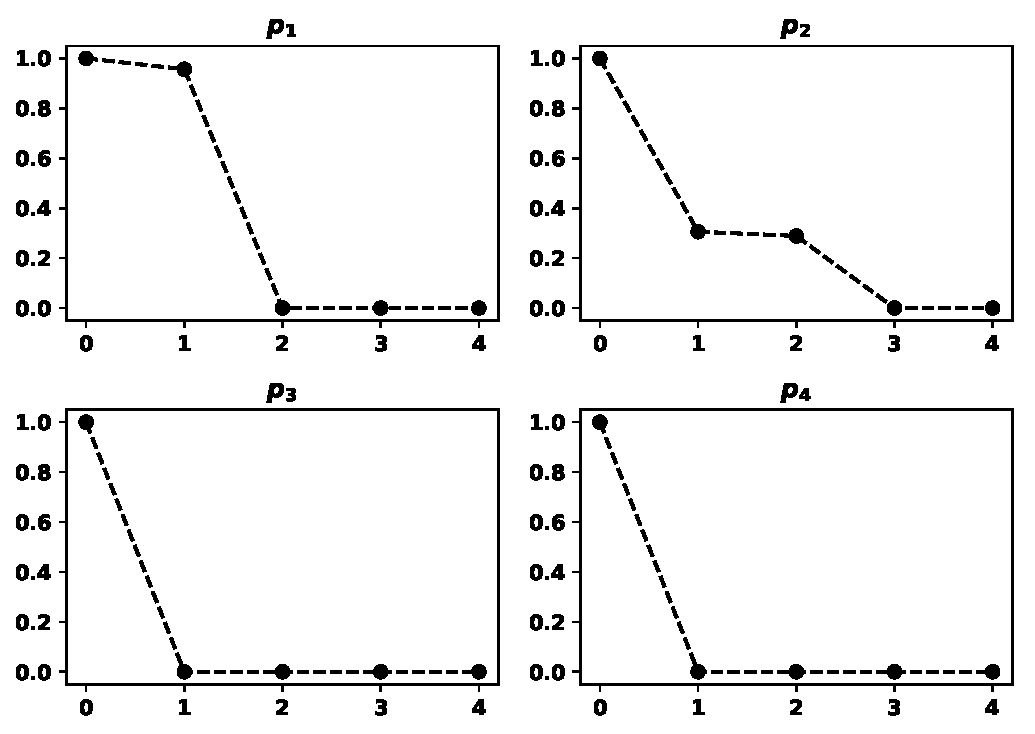
\includegraphics[width=.6\textwidth]{img/evolution_example_two.pdf}
    \caption{Best response dynamics with \(N=2\). More specifically, for
    \(q ^{(1)}=(0.2360,
                0.1031,
                0.3960,
                0.1549)\) and
    \(q ^{(2)}=(0.0665,
                0.4015,
                0.9179,
                0.8004)\).}
\label{fig:best_response_dynamics_results}
\end{figure}

For each pair of opponents, from the data set described in
Section~\ref{subsection:best_response_n_2} we have also recorder the evo
strategy. Thus, a total of 1000 different evos have been estimated. Similarly,
to previous results, the evos do not appear to behave in an extortionate way
either. Only 30\% have an SSerror less than a 0.1 and the distribution of error
has a large positive skewness \(=3.33\) indicating a longer tail to the right.
More and more strategies behave less and less extortionate
(Figure~\ref{fig:sserror_mem_one} and Table~\ref{table:sserror_stats}).

\begin{figure}
    \begin{minipage}{0.69\textwidth}
            \begin{center}
            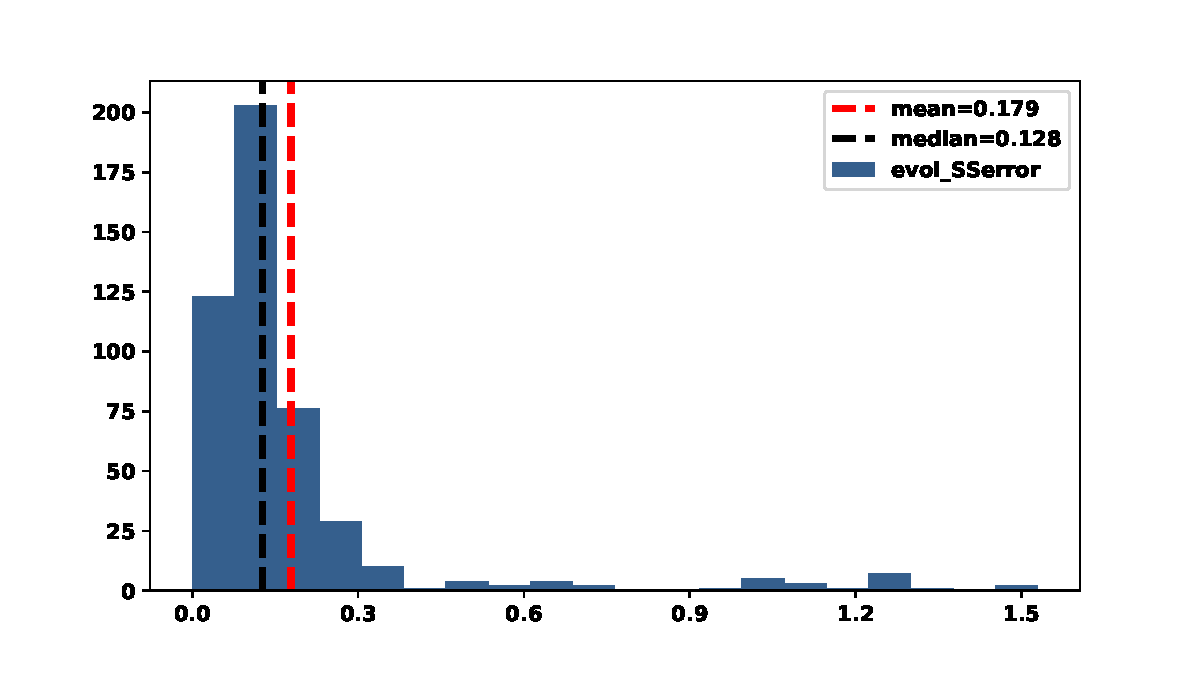
\includegraphics[width=.85\linewidth]{img/evo_sserror.pdf}
            \end{center}
            \caption{Distribution of sserrors for memory one best responses, when \(N=2\)}
            \label{fig:sserror_mem_one}
    \end{minipage}
    \hfill
    \begin{minipage}{0.29\textwidth}
        \centering
        \captionsetup{type=table}
        \resizebox{.61\columnwidth}{!}{%
            \begin{tabular}{lr}
\toprule
{} &  Evo SSerror \\
\midrule
count &  1023.000000 \\
mean  &     0.189929 \\
std   &     0.219760 \\
min   &     0.000000 \\
25\%   &     0.075918 \\
30\%   &     0.097995 \\
35\%   &     0.113404 \\
50\%   &     0.140975 \\
max   &     1.529412 \\
\bottomrule
\end{tabular}
}
            \caption{Summary statistics SSerror}
            \label{table:sserror_stats}
      \end{minipage}
\end{figure}

The majority of neither best response and evolutionary best response memory one
strategies are behaving in extortionate way. In order to understand the difference
between the two set of strategies we consider the distributions of their respective
transition probabilities, Figure~\ref{fig:behaviour_violin_plots}.
Though there is no significant difference between the medians of each
distribution, Table~\ref{table:wilcoxon_tests}, it is evident from Figure~\ref{fig:behaviour_violin_plots}
that there is variation in the behaviors.

Except from the case of \(p_3\):

\begin{itemize}
    \item If a
    strategy manages to get away with a defection, and receives a temptation payoff,
    the strategy will try another defection in the next round.  That is true for
    both best response memory one and evo.
\end{itemize}

For cases of \(p_1, p_2\) and \(p_4\):

\begin{itemize}
    \item After the \(CC\) state where a mutual cooperation has occur, best
    responses memory one strategies are either going to cooperate of defect,
    with very high probabilities. The are more likely however, to defect and
    break the cycle of cooperation. In comparison evos are more stochastic. The
    two extreme peaks do not appear in the case of evos, and overall there is a
    slightly bigger insensitive for cooperation from evos.
    \item In cases of \(CD\), a state that a strategy has been tricked, best
    response memory one strategies are very quick at punishing the strategy,
    they are interacting with. On the other hand evos are slightly more likely
    to cooperate again, to forgive their opponent. This could be a result of
    self interaction and evos and trying to not punish themselves.
    \item Finally, in cases that a mutual defection has occur, evos probability
    cooperating again is practically zero. Evos are not forgiving after a mutual
    defection, whereas best response strategies are.
\end{itemize}

The difference of between the transition probabilities of evos and best responses,
at each trial, is also given, Figure~\ref{fig:distances} to further our results.

\begin{figure}
    \centering
    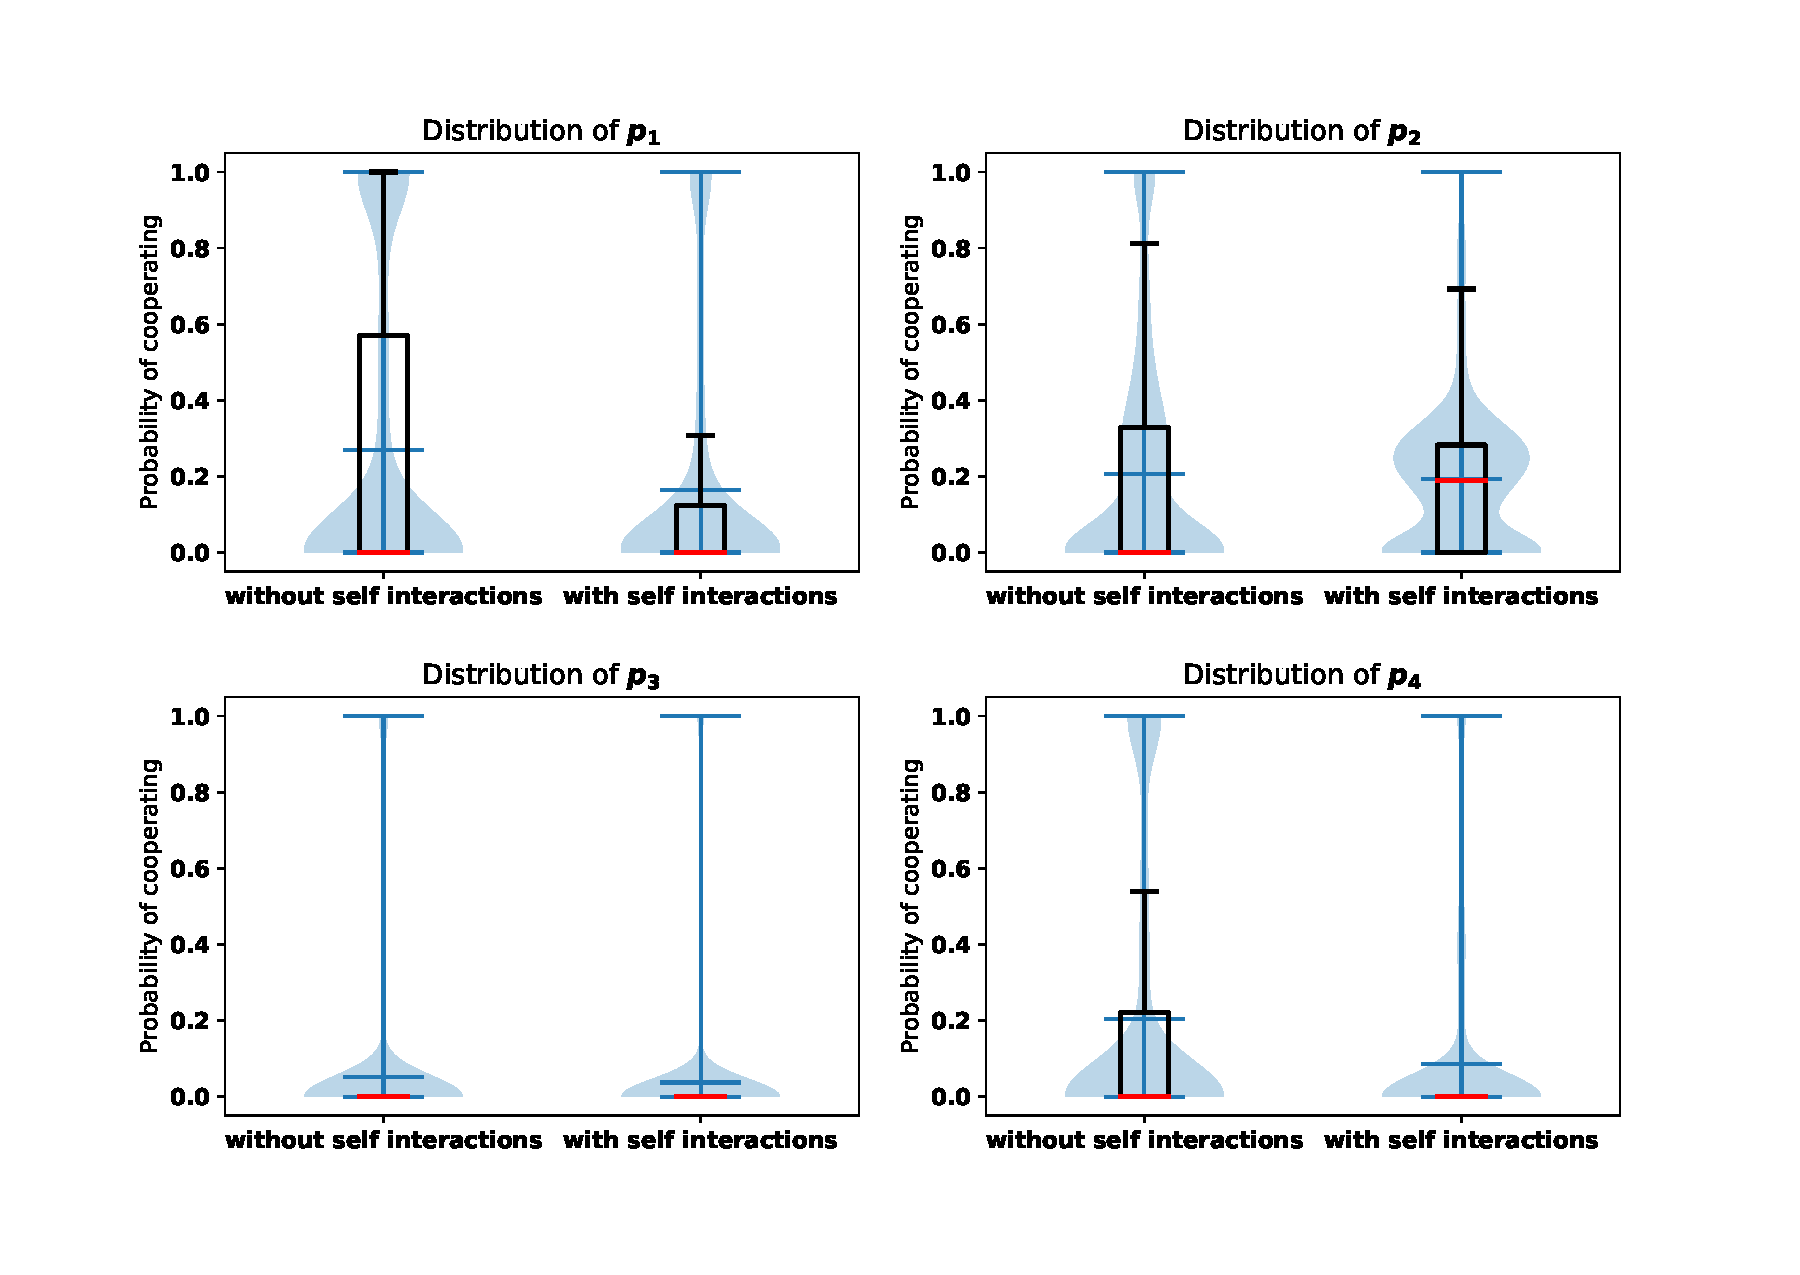
\includegraphics[width=.8\textwidth]{img/behaviour_violin_plots.pdf}
    \caption{Distributions of \(p\) for both best response and evo memory one
    strategies.}
    \label{fig:behaviour_violin_plots}
\end{figure}

\begin{table}
    \centering
    \resizebox{.41\columnwidth}{!}{%
    \begin{tabular}{lrrr}
\toprule
{} &  Memory one Median &  Evo Median &  p-values \\
\midrule
Distribution $p_1$ &                0.0 &    0.000000 &       0.0 \\
Distribution $p_2$ &                0.0 &    0.174359 &       0.0 \\
Distribution $p_3$ &                0.0 &    0.000000 &       0.0 \\
Distribution $p_4$ &                0.0 &    0.000000 &       0.0 \\
\bottomrule
\end{tabular}
}
    \caption{A non parametric test, Wilcoxon Rank Sum, has been performed to
    tests the difference in the medians. A non parametric test is used because
    is evident that out data are skewed.}\label{table:wilcoxon_tests}
\end{table}

\begin{figure}
    \centering
    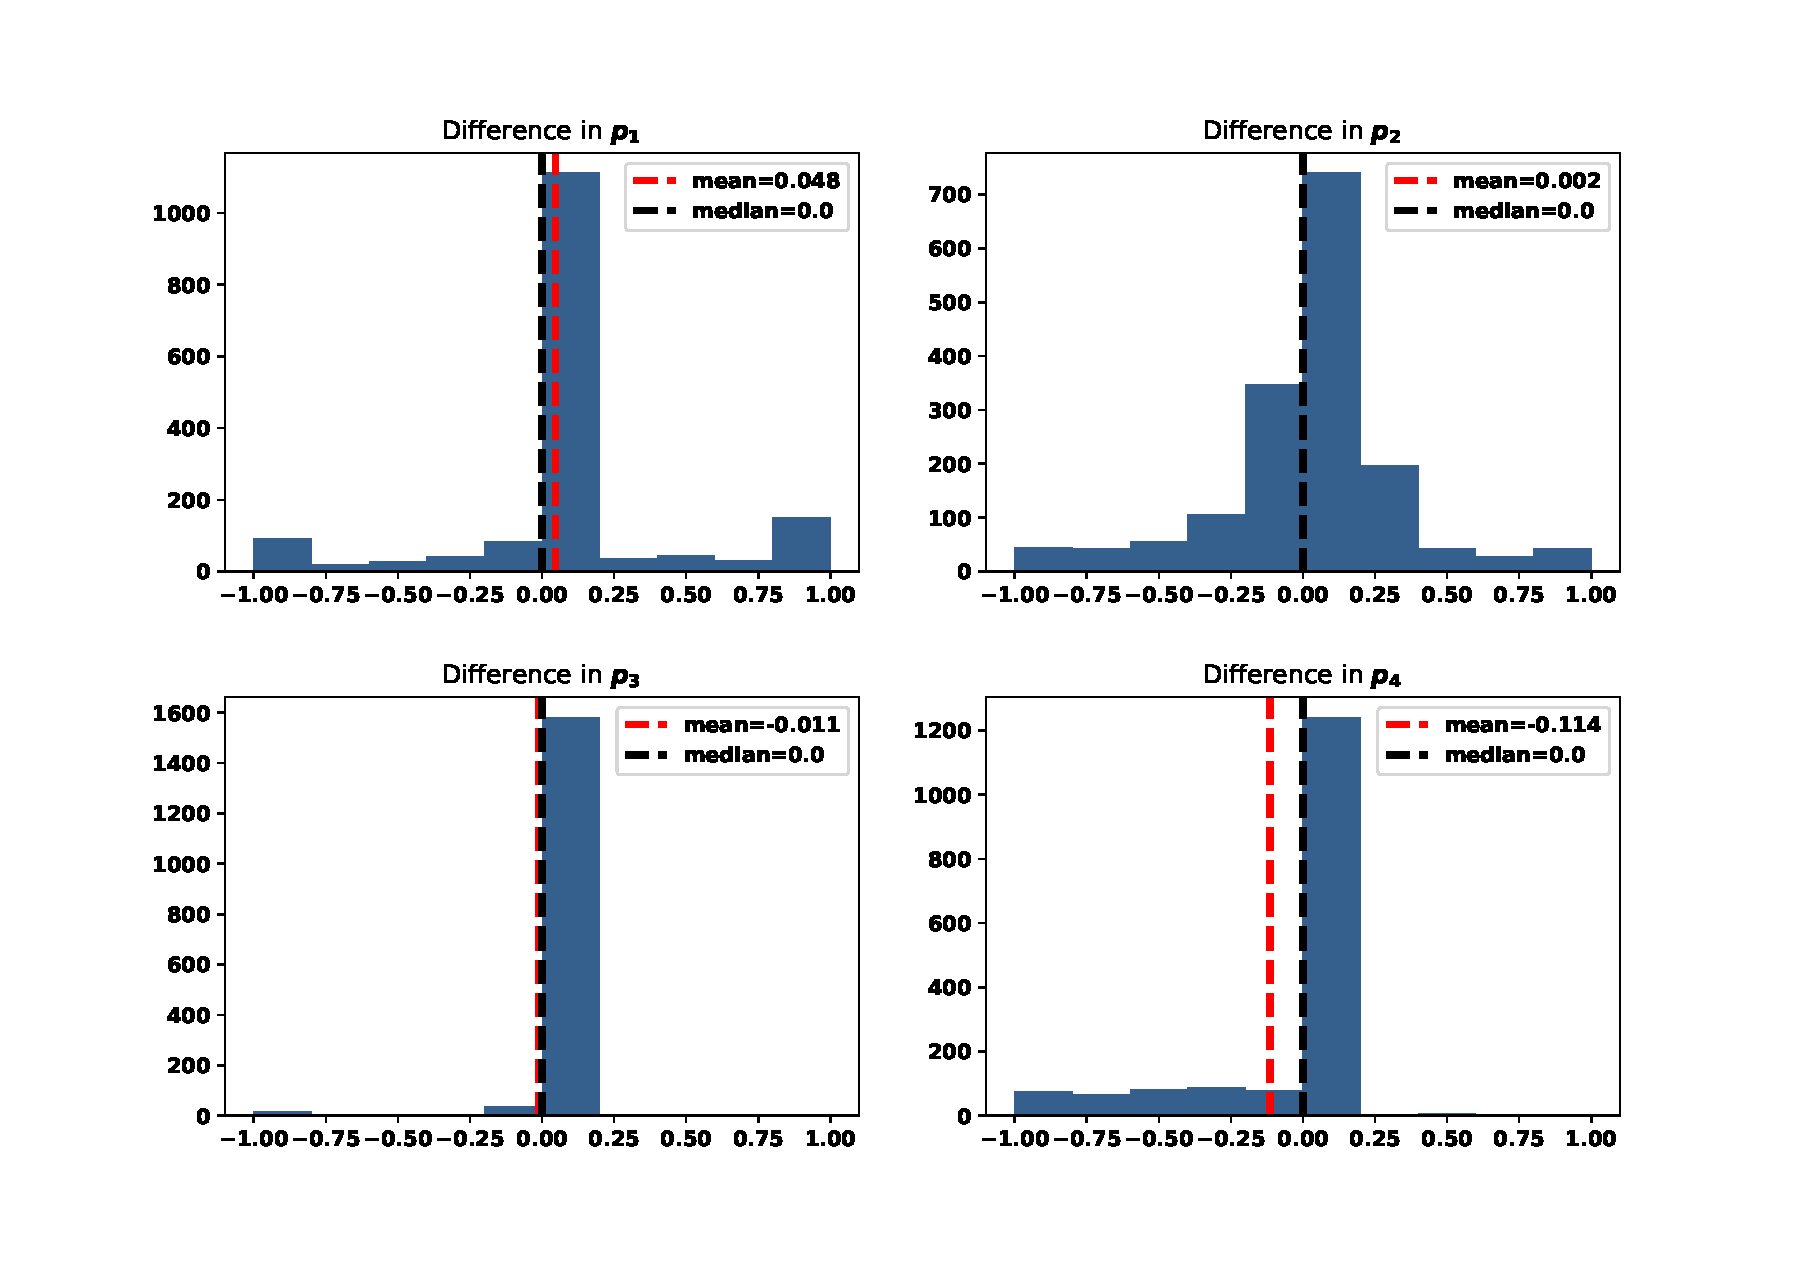
\includegraphics[width=.8\textwidth]{img/distances.pdf}
    \caption{Differences of \(p_(i)\) for \(i \in {1, 2, 3, 4}\) between evos and best responses at each trial.}
    \label{fig:distances}
\end{figure}


\section{Longer memory best response}

The third and final case considered in this paper focuses on proving that short memory strategies
have limitations. In this section we introduce several empirical results that
show that more complex strategies can indeed perform better in cases of \(N=2\).
This is achieved by comparing the performance of an optimised memory one strategy
to that of a trained long memory one.

The longer memory strategy we have chosen is a strategy called Gambler,
introduced and discussed in~\cite{Harper2017}. A Gambler strategy makes probabilistic
decisions based on the:

\begin{itemize}
    \item Opponent's first moves, \(n_1\).
    \item Opponent's last moves, \(m_1\).
    \item Player's last moves, \(m_2\)
\end{itemize}

This manuscript considers a Gambler($n_1 = 2, m_1 = 1, m_2 = 1$). By considering
the opponent's first more, the opponents last move and two of our own, there are
only 16 possible outcomes that can occur.

\includestandalone{tex/gambler_outcome}


Bayesian optimisation is used to estimate the cooperating probabilities for
a Gambler after each possible state plus the probability of starting with a 
cooperation. Gambler's utility is the estimated using~\cite{axelrodproject}
as the tournament result against two random opponents. The tournament is
run for. A total of 70 trails have been recorded and the data can be found here.

\begin{figure}
    \centering
    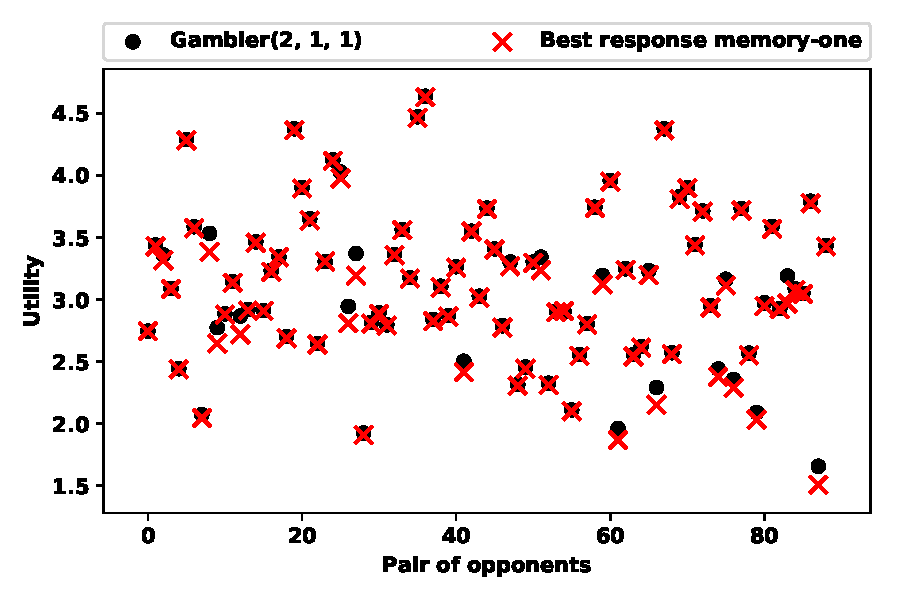
\includegraphics[width=.6\textwidth]{img/gambler_performance_against_mem_one.pdf}
\end{figure}

% \begin{figure}
%     \centering
%     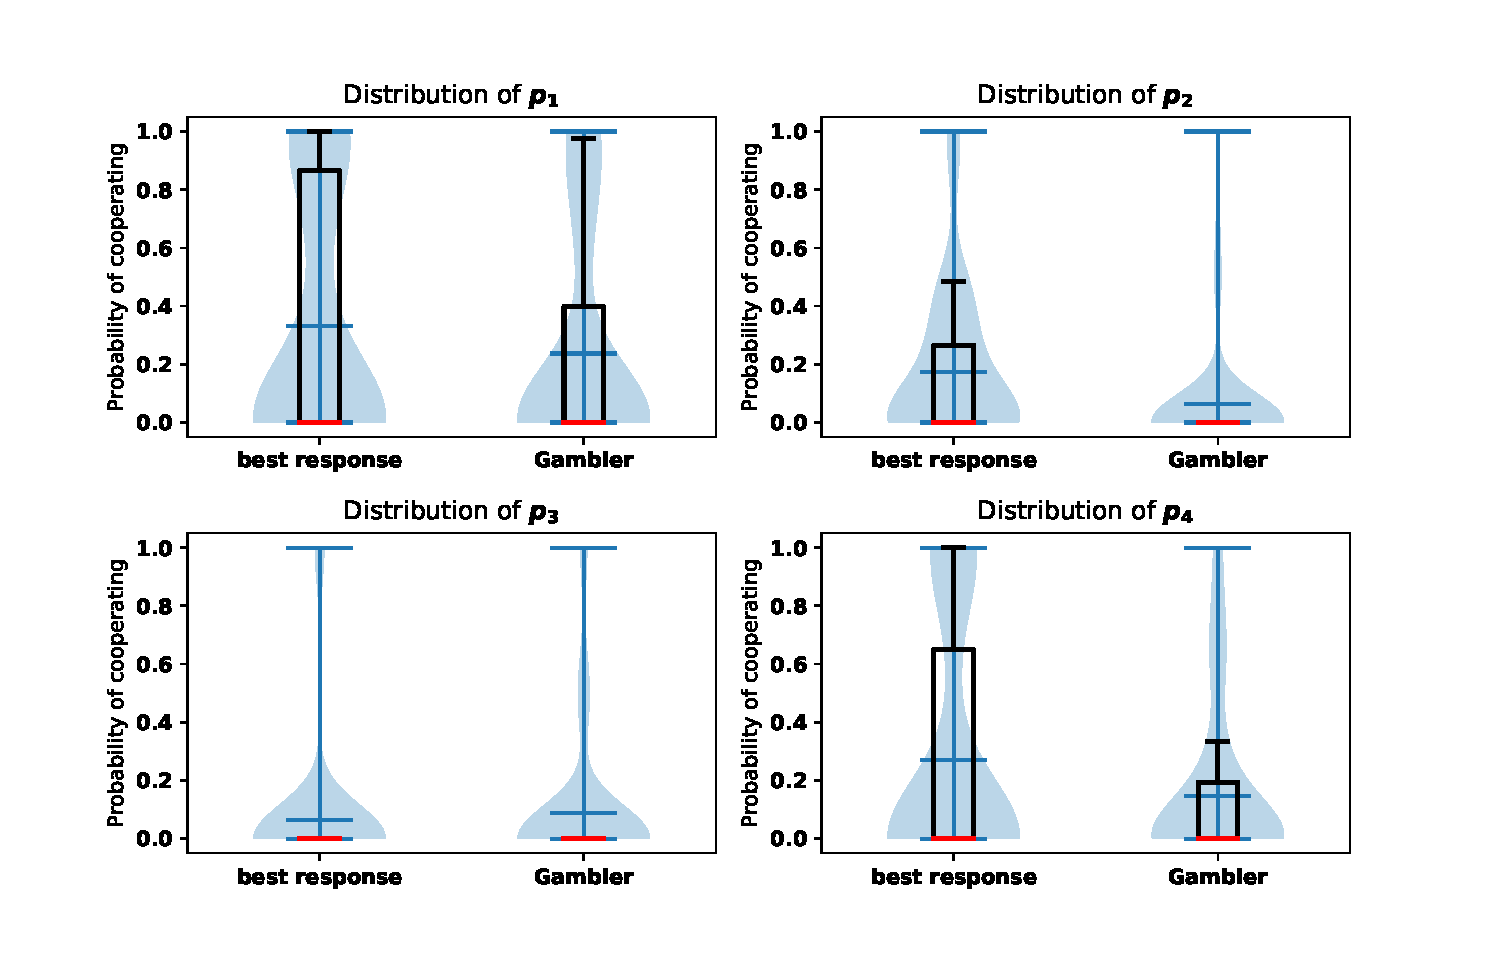
\includegraphics[width=\textwidth]{img/gambler_vs_mem_violinplot.pdf}
% \end{figure}


\section{Conclusion}


% Bibliography
\bibliographystyle{plain}
\bibliography{bibliography.bib}

\appendix
\section{Appendix Tables}\label{appendix:tables}

The memory one strategies used in the computer tournament described in~\cite{Stewart2012}
are given by Table~\ref{table:list_stewart_plotkin}.


\begin{table}
        \begin{center}
        \resizebox{.5\textwidth}{!}{\begin{tabular}{clcc}
        \toprule
        {}&  Name & Memory one representation & Reference \\
        \midrule
        1  & Cooperator           & \((1, 1, 1, 1)\) & \cite{Axelrod1981} \\
        2  & Defector             & \((0, 0, 0, 0)\) & \cite{Axelrod1981}\\
        3  & Random               & \((\frac{1}{2}, \frac{1}{2}, \frac{1}{2},
        \frac{1}{2})\) & \cite{Axelrod1981} \\
        4  & Tit for Tat          & \((1, 0, 1, 0)\) & \cite{Axelrod1981}\\
        5  & Grudger              & \((1, 0, 0, 0)\) & \cite{Li2011} \\
        6  & Generous Tit for Tat & \((1, \frac{1}{3}, 1, \frac{1}{3})\) & \cite{Nowak1990}\\
        7  & Win Stay Lose Shift  & \((1, 0, 0, 1)\) & \cite{Nowak1993} \\
        8  & ZDGTFT2              & \((1, \frac{1}{8}, 1, \frac{1}{4})\) &\cite{Stewart2012}\\
        9  & ZDExtort2            & \((\frac{8}{9}, \frac{1}{2}, \frac{1}{3},
        0)\) & \cite{Stewart2012}\\
        10 & Hard Joss            & \((\frac{9}{10}, 0, \frac{9}{10}, 0)\) &
        \cite{Stewart2012} \\
        \bottomrule
    \end{tabular}}
    \caption{List of strategies used in the tournament described in~\cite{Stewart2012}.}
    \label{table:list_stewart_plotkin}
    \end{center}
\end{table}
\end{document}

